% !TeX root = ../main.tex
\chapter{System Design}

System design in Jan-Sunwai AI focuses on reliable complaint orchestration in a governance-sensitive environment. The design balances modular API responsibilities, AI integration boundaries, role-specific UI behavior, and document-oriented persistence strategies.

\section{System Architecture Design}

System architecture design was developed to ensure clear separation of concerns while preserving end-to-end traceability across complaint intake, processing, and governance review. The design prioritizes predictable integration boundaries among frontend, backend, data, and AI runtime layers so that failures can be isolated and recovered without cascading disruption. This architecture also supports future scaling through modular service evolution [11, 12, 13, 17, 16].

\subsection{Architectural Style}

The platform follows a layered service architecture:

\begin{itemize}
\item Presentation Layer: React SPA with role-aware route protection.
\item API Layer: FastAPI routers grouped by domain concern.
\item Service Layer: Assignment, queueing, sanitization, and utility services.
\item Data Layer: MongoDB collections and indexes.
\item AI Runtime Layer: Ollama-hosted models with staged invocation.
\end{itemize}

\placeholderfigure{Overall System Context Diagram}{Users interact with the frontend, which communicates with backend APIs. Backend coordinates MongoDB, uploads storage, AI runtime, notification logic, and escalation loop.}

\placeholderfigure{Component Architecture Diagram}{Frontend modules map to backend routers and services. Persistence collections and model runtime are isolated behind service interfaces for maintainability and testability.}

\subsection{Key Architectural Decisions}

Key design decisions are summarized below:


\begin{table}[H]
\centering
\begin{tabularx}{\textwidth}{|p{0.33\textwidth}|X|}
\toprule
\textbf{Decision} & \textbf{Rationale} \\ \hline
\midrule
Hybrid AI pipeline (vision + rules + optional reasoning) & Reduces hallucination risk, lowers VRAM pressure, and improves deterministic routing for common civic scenes \\ \hline
Document model in MongoDB & Supports rich complaint lifecycle payloads and embedded audit metadata without heavy relational join overhead \\ \hline
Role-specific route gates & Enforces operational boundaries between citizen, worker, department head, and admin personas \\ \hline
Queue-based draft generation fallback & Prevents long-running model calls from blocking frontend experience \\ \hline
Security middleware and sanitization by default & Reduces exploit surface for API consumers and file uploads \\ \hline
Versioned API alias (/api/v1) & Improves long-term integration stability for external municipal consumers \\ \hline
\bottomrule
\end{tabularx}
\caption{Major Design Decisions and Rationale}
\label{tab:design-decisions}
\end{table}

\subsection{AI Classification Pipeline}

To ensure reliable routing, the AI component employs a hybrid model combining vision-language inference with deterministic thresholding. When an image is uploaded, the vision model generates class probabilities. The final confidence score is formulated as the maximum probability across predefined civic categories:

\begin{equation}
\text{Confidence} = \max_{i} (P(\text{class}_i \mid \text{image}))
\end{equation}

If this $\text{Confidence}$ exceeds the system's acceptable threshold (e.g., $0.70$), the complaint is auto-routed to the corresponding department. If the confidence falls below this threshold, the system flags the submission for the administrative triage queue, ensuring human oversight handles ambiguous cases.

\section{UML Diagrams}

The following diagrams are aligned with the implemented module boundaries, routing flow, and lifecycle stages documented in the project report and API references.

\subsection{E-R Diagram}

\placeholderfigure{E-R Diagram}{Primary entities: User, Complaint, Notification, and PasswordReset token. Relationships include complaint ownership, assignment, and notification generation.}

\textbf{Data Flow \& Rationale:} This diagram shows how complaint records act as the central nexus linking users, workers, and notifications. By embedding status history directly within the Complaint entity, the database minimizes costly relational joins during dashboard rendering.

\subsection{Use Case Diagram}

\placeholderfigure{Use Case Diagram}{Citizen submits and tracks complaints; worker resolves assignments; department head updates status; admin governs approvals, triage, and analytics.}

\textbf{Role Segregation \& Governance:} This diagram captures the strict access boundaries enforced by the system. While citizens have broad permission to create and track records, state mutations (such as resolving or rejecting a complaint) are heavily restricted to authenticated workers and department heads. It visually demonstrates the governance principle that AI assists but humans hold final approval authority.

\subsection{Class Diagram}

\placeholderfigure{Class Diagram}{Schema-level classes represent User, Complaint, and Notification with association to role, status, and metadata properties.}

\textbf{Data Encapsulation:} The class structure reflects the document-oriented database design where complex types like Geolocation and Timestamps are embedded rather than relationally linked. This tradeoff sacrifices some normalization but ensures that fetching a single Complaint object provides the frontend with the complete operational context needed to render a dashboard.

\subsection{Sequence Diagram}

\placeholderfigure{Sequence Diagram}{Upload -> analyze -> generate draft -> submit complaint -> auto-assign -> status updates -> notifications.}

\textbf{Flow \& Bottlenecks:} This sequence outlines the chronological journey of a grievance. It highlights the AI inference step as the primary synchronous bottleneck. To prevent browser timeouts, the system restricts the analysis time window and degrades gracefully to a manual form if inference times out.

\subsection{Activity Diagram}

\placeholderfigure{Activity Diagram}{Lifecycle from citizen intake through operational processing and closure with feedback and audit logging.}

\textbf{State Machine Constraints:} This diagram tracks the rigid state transitions a complaint undergoes (e.g., from `Pending` to `In Progress` to `Resolved`). It illustrates the system's fail-safes: if the AI classification confidence is low, the activity branches into the administrative triage queue rather than failing silently, preventing black-hole scenarios in civic reporting.

\subsection{DFD Diagram}

\placeholderfigure{Data Flow Diagram}{Data moves from frontend to API services, then to persistence and AI runtime. Notification and analytics streams derive from lifecycle events.}

\textbf{System Dynamics:} The DFD maps the transition of unstructured citizen uploads into structured database records. It illustrates why the AI module is isolated from the core CRUD API—allowing the transaction engine to operate independently of the compute-heavy vision processing.

\subsection{Deployment Diagram}

\placeholderfigure{Deployment Diagram}{Browser clients access frontend service; frontend proxies API calls to backend service; backend communicates with MongoDB and host-level Ollama runtime.}

\textbf{Local-First Architecture:} The deployment topology explicitly avoids managed cloud dependencies to comply with municipal security constraints. By keeping the React bundle, FastAPI server, MongoDB, and Ollama LLM isolated within a Docker Compose network, the diagram proves that the entire grievance platform can be air-gapped or run on constrained on-premises infrastructure.

\section{Database Design}

Database design focused on lifecycle integrity, query efficiency, and auditability rather than strict relational normalization. Since complaint records evolve through multiple state transitions and actor interactions, the chosen document model keeps operationally related history close to primary complaint entities while retaining key references for role and ownership controls. This approach improves retrieval speed for dashboards, timelines, and governance reviews [13, 11, 14].

\subsection{Table Design and Relationships}

The database is organized around four principal collections:

\begin{itemize}
\item \textbf{users}: identity, role, and worker service-area metadata.
\item \textbf{complaints}: complaint payload, routing metadata, status history, and collaboration artifacts.
\item \textbf{notifications}: user-scoped notification events and read-state tracking.
\item \textbf{password\_resets}: token hash lifecycle with expiry and usage state.
\end{itemize}

The design intentionally keeps lifecycle and audit structures close to complaint documents for locality and retrieval simplicity.

\subsection{Normalization}

The platform uses controlled denormalization:

\begin{itemize}
\item Embedded \texttt{status\_history}, \texttt{dept\_notes}, and \texttt{comments} reduce query complexity.
\item Core identity references (e.g., \texttt{user\_id}, \texttt{assigned\_to}) remain external for role and profile updates.
\item Routing metadata is persisted with complaint records to preserve deterministic decision context over time.
\end{itemize}

This approach preserves operational read performance while retaining clear ownership semantics.

\subsection{Indexing Strategy}

Key indexing strategies are summarized below:


\begin{table}[H]
\centering
\begin{tabularx}{\textwidth}{|p{0.22\textwidth}|p{0.31\textwidth}|X|}
\toprule
\textbf{Collection} & \textbf{Index} & \textbf{Purpose} \\ \hline
\midrule
users & unique(username), unique(email) & Fast auth lookups and uniqueness enforcement \\ \hline
complaints & (user\_id, created\_at) & Efficient citizen dashboard history retrieval \\ \hline
complaints & (status, created\_at) & Queue and status-oriented admin filtering \\ \hline
complaints & (department, created\_at) & Department-level operational listing \\ \hline
complaints & authority\_id & Escalation and authority review queries \\ \hline
notifications & (user\_id, created\_at) & Ordered notification feed retrieval \\ \hline
notifications & (user\_id, is\_read) & Unread badge counter queries \\ \hline
\path{password_resets} & \path{unique(token_hash)} & Token lookup and collision prevention \\ \hline
\path{password_resets} & \path{(user_id, used)} & Active token invalidation management \\ \hline
\path{password_resets} & \path{TTL(expires_at)} & Automatic expired-token cleanup \\ \hline
\bottomrule
\end{tabularx}
\caption{Indexing Strategy by Collection}
\label{tab:indexing-strategy}
\end{table}

\section{GUI Design}

GUI design was planned as a task-oriented interface model where each role sees only the controls and data required for its responsibilities. Visual hierarchy, workflow clarity, and responsive behavior were treated as core functional requirements because field and supervisory users interact with the platform under different device and time constraints. The resulting interface strategy emphasizes speed of action, low ambiguity, and consistent feedback.

\subsection{Design Principles}

The UI follows practical governance portal principles:

\begin{itemize}
\item Clarity of action over decorative complexity.
\item Explicit role boundaries in navigation and controls.
\item Immediate visual feedback for status and notification changes.
\item Responsive behavior for desktop operator screens and mobile field usage [21].
\end{itemize}

\subsection{Interface Areas}

Key interface areas are summarized below:


\begin{table}[H]
\centering
\begin{tabularx}{\textwidth}{|p{0.25\textwidth}|X|}
\toprule
\textbf{Interface Area} & \textbf{Purpose} \\ \hline
\midrule
Public Home & Awareness, role entry points, and transparency access \\ \hline
Authentication Screens & Login, registration, forgot password, reset password \\ \hline
Analyze and Result Views & Upload, AI analysis display, map interaction, draft review \\ \hline
Citizen Dashboard & Complaint list, timeline, feedback, and progress visibility \\ \hline
Worker Dashboard & Assigned queue and completion updates \\ \hline
Department Head Dashboard & Department-level filtering, status updates, and notes \\ \hline
Admin Dashboard & Global queue, approvals, triage, bulk actions, analytics, exports \\ \hline
Notification Panel & Event feed and read-state management \\ \hline
Profile Screen & Personal information update controls \\ \hline
\bottomrule
\end{tabularx}
\caption{GUI Areas and Purpose}
\label{tab:gui-areas-purpose}
\end{table}

\subsection{Wireframe Reference}

The following figure provides a visual reference that complements the explanatory text in this subsection.


\begin{figure}[H]
\centering
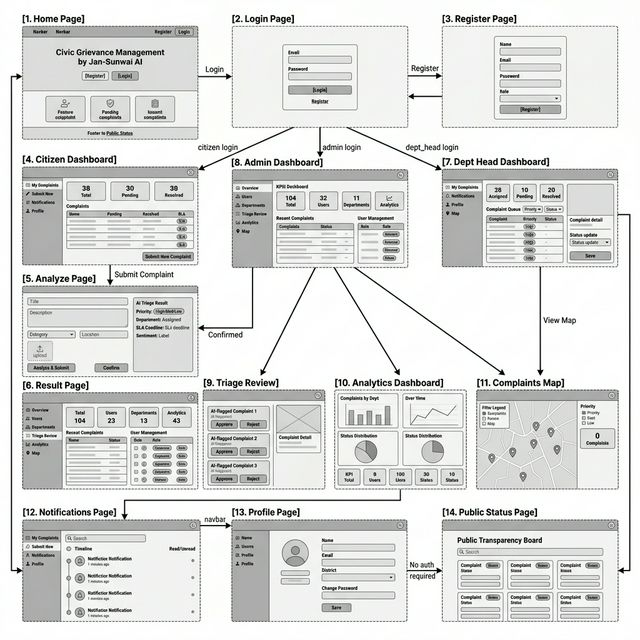
\includegraphics[width=0.85\textwidth]{../../images/GUI_Wireframe.png}
\caption{GUI Wireframe Reference from Project Documentation}
\label{fig:gui-wireframe}
\end{figure}

\section{Screenshots}

The screenshot gallery below restores representative evidence from the implementation while keeping the report compact enough for submission.

\begin{center}
\screenshotcard[S01: Home Page Hero]{0.47\textwidth}{fig:s01}{../../images/screenshots/S01_home_desktop.png}{S01: Home Page Hero and Public Entry CTA}\hfill
\screenshotcard[S02: AI Analysis Result]{0.47\textwidth}{fig:s02}{../../images/screenshots/S02_analyze_result.png}{S02: AI Analysis Result and Draft Review}
\end{center}

\vspace{1em}

\begin{center}
\screenshotcard[S03: Citizen Tracking Dashboard]{0.47\textwidth}{fig:s03}{../../images/screenshots/S03_citizen_dashboard.png}{S03: Citizen Complaint Tracking Dashboard}\hfill
\screenshotcard[S04: Worker Assignment Queue]{0.47\textwidth}{fig:s04}{../../images/screenshots/S04_worker_dashboard.png}{S04: Worker Assignment Queue}
\end{center}

\vspace{1em}

\begin{center}
\screenshotcard[S05: Admin Dashboard]{0.47\textwidth}{fig:s05}{../../images/screenshots/S05_admin_dashboard_desktop.png}{S05: Admin Dashboard --- shows real-time complaint volume, department breakdown, and pending approvals. The admin can initiate bulk status updates or export records from this single view.}\hfill
\screenshotcard[S06: Admin Triage Queue]{0.47\textwidth}{fig:s06}{../../images/screenshots/S06_triage_queue.png}{S06: Administrative Triage Queue --- displays low-confidence AI classifications awaiting human review. The confidence score, AI-suggested category, and uploaded image are shown side-by-side so the admin can approve, reject, or relabel in one action.}
\end{center}

\section{Chapter Summary}

This chapter defined structural design choices, module interactions, data modeling strategy, and UI architecture. The design emphasizes traceability, secure operations, and practical maintainability while accommodating AI-assisted workflows in a municipal governance context.
